\subsection{Ray Marching}
\label{subsec:ray_marching}

~\citeauthor{perlin_hypertexture_1989} schlagen eine Abtastung des
Strahles mit fixen Abständen $\Delta \mu$ vor~\parencite[S.
259]{perlin_hypertexture_1989}:

\begin{gather}
    x = x_{\mu_{0}} + k \cdot \Delta x_{\mu}
\end{gather}

wobei $k = 0,1,2,\dots$ und $\mu_{0} + k \Delta \mu \leq \mu_{1}$ ist.

Auf die parametrische Darstellung eines (Licht-) Strahles,
~\autoref{eq:ray_param_cond}, angewendet, ergibt dies folgende Gleichung:

\begin{gather}
    r(k) = r_{0} + \Delta t \cdot k \cdot r_{d}
\end{gather}

wobei $\Delta t$ die Grösse der Abstände und $k = 0,1,2,\dots$ die Nummer der
Schritte darstellt. Wie~\citeauthor{hart_ray_1989} schreiben, bildet das Abtasten des
(Licht-) Strahles mit fixen Abständen die Basis für gewisse Verfahren des
volumetrischen Renderings~\parencite[S. 291]{hart_ray_1989}.

Ein möglicher Algorithmus, wie solch ein Verfahren umgesetzt werden kann,
findet sich in~\autoref{fig:ray_marching}.

\begin{lstlisting}[language=Python,caption={Eine abstrakte Umsetzung des Ray
        Marchings\protect\footnotemark.},label={fig:ray_marching},captionpos=b,emph={ray_march}]
def ray_march():
    step         = 0
    intersection = 0
    max_steps    = 10

    while step < max_steps:
        intersection = test_intersection(k)

        if intersection <= 0:
            # An intersection has happened
            #   intersection <  0: ray is inside surface
            #   intersection == 0: ray is excatly on surface
            return ray_travel_distance(step)

        step = step + 1

    # When we reach this step, after max_steps, no intersection
    # has happened, so distance is 0
    return 0
\end{lstlisting}
\footnotetext{Algorithmus in Pseudocode
    gemäss~\cite{perlin_hypertexture_1989}[S. 259, Abschnitt 3.1]}

Dabei ist jedoch zu beachten, dass der Abstand zur Abtastung eines Strahles
$\Delta t$ so gering als möglich sein sollte um eine Menge von Punkten bzw.\ ein
Objekt --- definiert durch implizite Oberflächen --- $A$ möglichst gut
abschätzen zu können. Ist der gewählte Abstand zu gross gewählt, so findet ggf.
eine Abtastung weit im Inneren des Objektes statt und somit geht Präzision
verloren.  Es ist auch möglich dass der erste eigentliche Punkt gar nicht
abgetastet wird und erst der zweite abgetastete Punkt das Objekt ``erkennt''.

\begin{figure}[H]
    \centering
    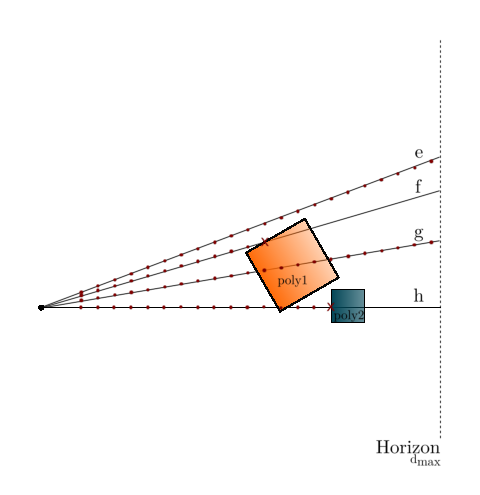
\includegraphics{img/ray_marching_problems.pdf}
    \caption{Illustration des Ray Marching Verfahrens und dessen
        Problematiken.\protect\footnotemark}\label{fig:ray_marching_problems}
\end{figure}
\footnotetext{Eigene Darstellung mittels Inkscape.}

\autoref{fig:ray_marching_problems} veranschaulicht diese
Problematiken. Zu sehen sind vier Primärstrahlen, \textit{e},
\textit{f}, \textit{g} und \textit{h},  sowie zwei Objekte,
\textit{poly1} und \textit{poly2}.

Bei den Strahlen \textit{e} und \textit{f} handelt es sich um
``normale'' Fälle: Der Strahl \textit{e} geht komplett an den Objekten
vorbei, das Ray Marching wird also nach erreichen der maximalen Distanz
\textit{d\textsubscript{max}} abgebrochen, der Strahl \textit{f} trifft
das Objekt \textit{poly1} nach 12 Schritten.

Bei den Strahlen \textit{g} und \textit{h} handelt es sich um
Spezialfälle: Der Strahl \textit{g} trifft das Objekt \textit{poly1}
nicht, obwohl der Strahl durch das Objekt hindurch geht. Dies geschieht
aufgrund der gewählten Distanz zum Abtasten der Strahlen ($\Delta t$).

Der Strahl \textit{h} trifft das Objekt \textit{poly2}, obwohl er
eigentlich das Objekt \textit{poly1} treffen müsste. Das getroffene
Objekt \textit{poly2} dürfte so gar nicht zu sehen sein. Dieser Fehler
tritt wiederum aufgrund der gewählten Distanz zur Abtastung der
Strahlen ($\Delta t$) auf.

\citeauthor{hart_sphere_1994} weist darauf hin, dass Ray Marching durch
den möglichst geringen Abstand zwischen den Abtastungen entsprechend
langsam und paralleles Abtasten praktisch unumgänglich ist~\parencite[S.
528]{hart_sphere_1994}. In der von~\citeauthor{hart_sphere_1994} vorgestellten
Technik des Sphere Tracings ist der Abstand zwischen den Abtastungen
nicht konstant sondern variiert in Abhängigkeit der
Geometrie~\parencite[S. 538 bis 540]{hart_sphere_1994}.
